
% 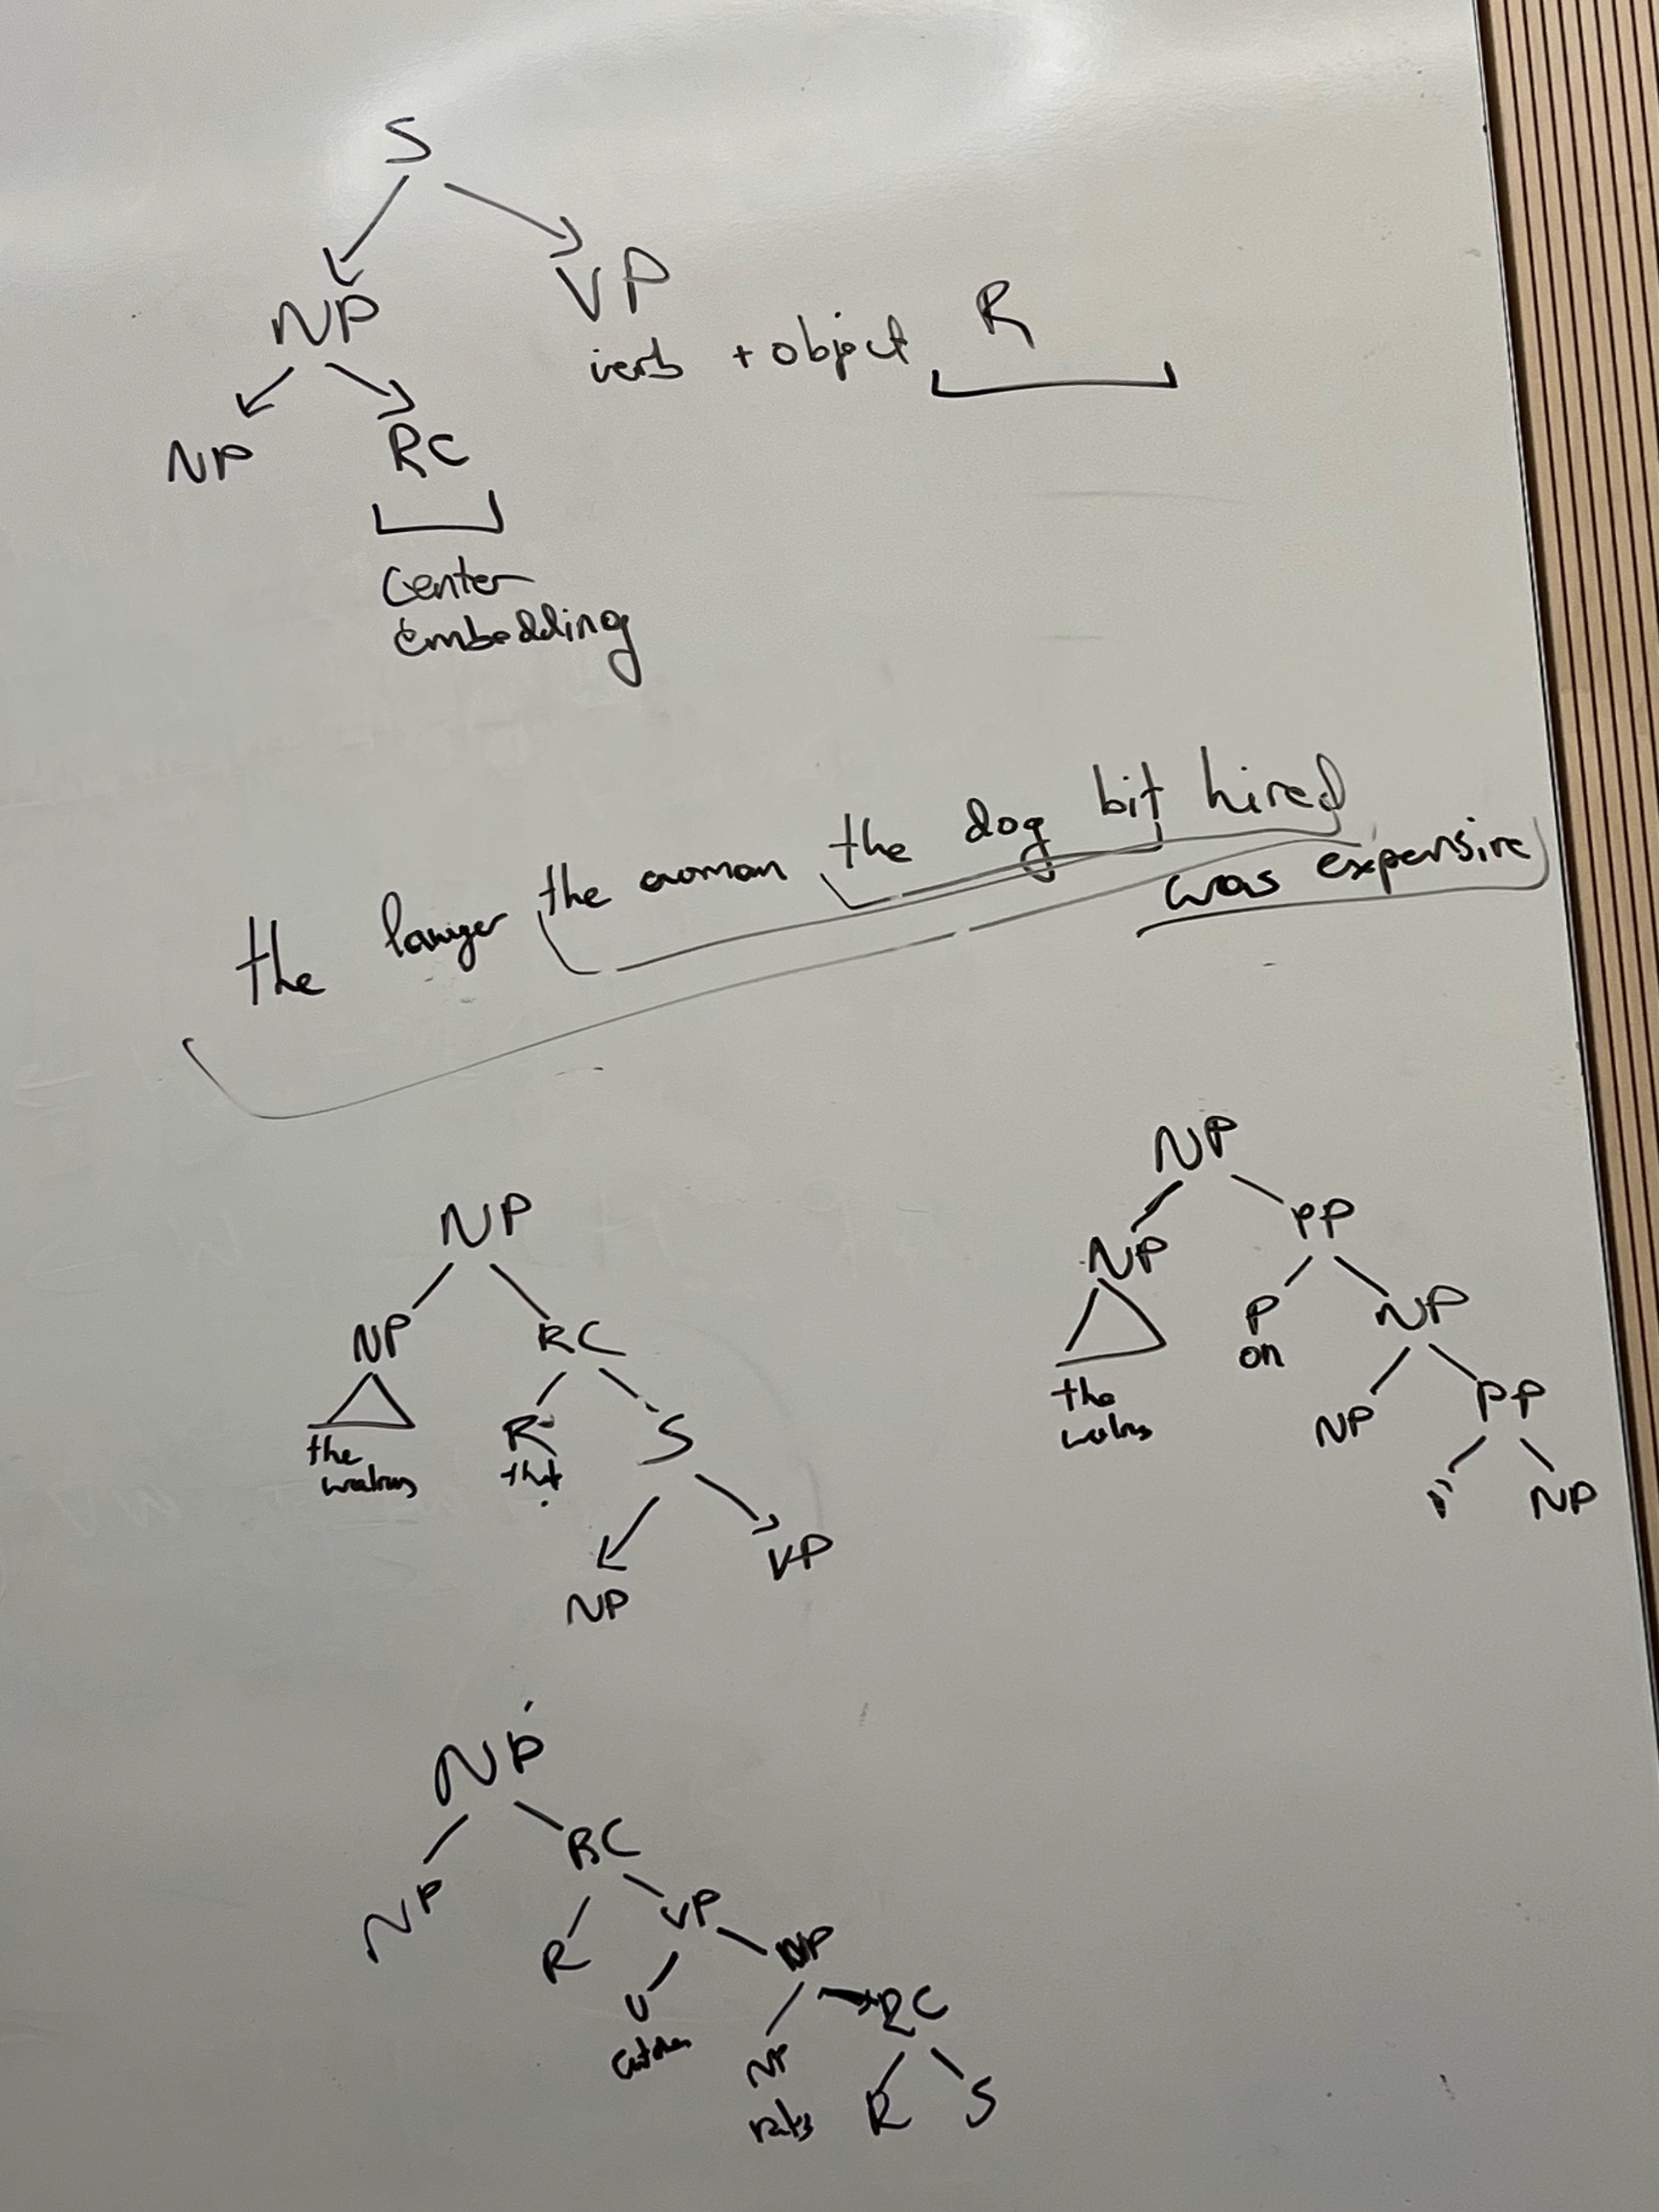
\includegraphics[width=0.48\textwidth]{figures/center_embed_demo.jpeg}


% \includegraphics[width=1.0\textwidth]{figures/test_acc_analysis_D280_52714736.png}
% \includegraphics[width=1.0\textwidth]{figures/test_acc_analysis_D281_52716914.png}
% \includegraphics[width=1.0\textwidth]{figures/test_acc_analysis_D283_52717479.png}
% \includegraphics[width=1.0\textwidth]{figures/test_acc_analysis_D284_52695892.png}

% Oct 23 Meeting updates:
% \begin{enumerate}
%     \item Question Formation:
%     \begin{enumerate}
%         \item Train only on center-embded decl leads to very consistent generalization
%         \item Unexpected: We initially suspect that we can introduce center-embeded decl in the question formation task, and thus get rid of the auxiliary task. But it turns out not to be the case. Model NEEDs to seem examples where the first auxiliary and the main auxiliary differ.
%         \item memorization: see appendix
%     \end{enumerate}
%     \item  Tense Inflection:
%     \begin{enumerate}
%         \item Now switch to a new way of presenting: (1) show that center-emebded sentences generalize hierarchically (2) Show that right-branching sentences don't. (3) Finally, show that with sufficient amount of center-embeded sentences, right-branching sentences can also generalize hieratically. Furthermore, the use of auxiliary task facilitate sentence type OOD generalization 
%         \item Looked into the evaluation objective - the default one, even though it is slightly weird is consistent with some other alternatives I tried. 
%     \end{enumerate}
%     \item Figure 1 alternative version. 
% \end{enumerate}


\section{Related Work Extended}
\label{appdx:related}
\subsection{Syntax and Hierarchical Generalization}
While works mentioned in Section \ref{sec:syntax_related} focused on models trained from scratch, another line of research examined the inductive bias of pretrained models. \citet{Mueller2024-qz, Mueller2023-xq} pretrained transformers on text corpora such as Wikipedia and CHILDES \citep{MacWhinney2014-jq} before fine-tuning them on the question formation task. They found that exposure to large amounts of natural language data enables transformers to generalize hierarchically.


Instead of using the question formation task as a probe, \citet{Hewitt2019-fc, Murty2022-lw} directly interpreted model's internal representation to understand whether transformers constrain their computations to to follow tree-structure patterns. \citet{Hewitt2019-fc} demonstrated that the syntax tress are embedded in model's representation space. Similarly, \citet{Murty2022-lw} projects transformers into a tree-structured network, and showed that transformers become more tree-like over the course of training on language data. 

\citet{Papadimitriou2023-gj, Papadimitriou2020-la} and \citet{Mueller2022-rm} also studied how pretraining data could introduce an inductive bias in language acquisition. \citet{Papadimitriou2023-gj} specifically identified that by pretraining models on data with a recursive structure  their performance when later finetuning them on natural language. This finding is closely related to our conclusions around the importance of recursive center embeddings. 



% \paragraph{Random variation} 
\subsection{Random Variation}
Specific training choices, such as hyperparameters, are crucial to model outcomes. However, even when controlling for these factors, training machine learning models remains inherently stochastic—models can be sensitive to random initialization and the order of training examples. \citet{Zhou2020-xt, D-Amour2022-tl, Naik2018-og} reported significant performance differences across model checkpoints on various analysis and stress test sets. \citet{Zhou2020-xt} further found that instability extends throughout the training curve, not just in final outcomes. To investigate the source of this inconsistency, \citet{Dodge2020-pb} compared the effects of weight initialization and data order, concluding that both factors contribute equally to variations in out-of-sample performance.


Similarly, \citet{Sellam2021-rz} found that repeating the pre-training process on BERT models can result in significantly different performances on downstream tasks. To promote more robust experimental testing, they introduced a set of 25 BERT-BASE checkpoints to ensure that experimental conclusions are not influenced by artifacts, such as specific instances of the model. In this work, we also observe training inconsistencies across runs on OOD data, both during training and at convergence. Unlike prior studies that focus on implications of random variations on experimental design, we study the source of training inconsistencies and link these inconsistencies to simplicity bias and the characteristics of the training data.



% \paragraph{Simplicity bias} 
\subsection{Simplicity Bias}
Models often favor simpler functions early in training, a phenomenon known as simplicity bias \citep{Hermann2020-ja}, which is also common in LMs. \citet{Choshen2022-qj} found that early LMs behave like n-gram models, and \citet{Saphra2019-sq} observed that early LMs learn simplified versions of the language modeling task. \citet{McCoy2019-br} showed that even fully trained models can rely on simple heuristics, like lexical overlap, to perform well on Natural Language Inference (NLI) tasks. \citet{Chen2023-fi} further explored the connection between training dynamics and simplicity bias, showing that simpler functions learned early on can continue to influence fully trained models, and mitigating this bias can have long-term effects on training outcomes.


Phase transitions have been identified as markers of shifts from simplistic heuristics to more complex model behavior, often triggered by the amount of training data or model size. In language models, \citet{Olsson2022-ed} showed that the emergence of induction heads in autoregressive models is linked to handling longer context sizes and in-context learning. Similar phase transitions have been studied in non-language domains, such as algorithmic tasks \citep{Power2022-hz, Merrill2023-an} and arithmetic tasks \citep{Nanda2023-zm, Barak2022-ub}.


In the context of hierarchical generalization, \citet{Ahuja2024-ul} used a Bayesian approach to analyze the simplicity of hierarchical versus linear rules in modeling English syntax. They argued that transformers favor the hierarchical rule because it is simpler than the linear rule. However, their model fails to explain (1) why learning the hierarchical rule is delayed (i.e., after learning the linear rule) and (2) why hierarchical generalization is inconsistent across runs. In this work, we offer a different perspective, showing that a model's simplicity bias towards either rule is driven by the characteristics of the training data.

